\chapter{Clustering von Bewegungsdaten mittels Dynamic Time Warping}
\label{chapter3}

Nach den einführenden Bemerkungen in \autoref{chapter1} und \autoref{chapter2} werden nun
die eingesetzten deterministischen Algorithmen näher beschrieben.
Die Grundlagen der Verfahren werden erläutert und an einem Beispiel veranschaulicht.
Ein Einblick in verwandte Arbeiten (\autoref{3-RelatedWork}) vertieft das Verständnis weiter.
Abschließend wird auf zu beachtende Besonderheiten des Kinect-Datensatzes eingegangen.

\section{Hierarchisches Time-Series Clustering}
\label{3-Clustering}
\emph{Clustering} kann genutzt werden, um große Datensätze zu kategorisieren,
wenn vorab keine Informationen über die Kategorien vorliegen \citep{aghabozorgi_time-series_2015}.
Ziel ist es, eine Struktur in den vorliegenden Daten zu finden,
indem Elemente anhand eines festgelegten Vorgehens in homogene Gruppen einsortiert werden.
Dabei sollen die Unterschiede bei Elementen der gleichen Gruppe möglichst klein
und bei Elementen verschiedener Gruppen möglichst groß sein \citep{aghabozorgi_time-series_2015, warren_liao_clustering_2005}.
Bei \emph{n} Datenpunkten erzeugt ein \emph{Clustering} \emph{k} Partitionen des Datensatzes.
Jede Partition entspricht dabei einem Cluster das mindestens ein Objekt enthält \citep{warren_liao_clustering_2005}.
Beim \emph{Clustering} sind besonders die Wahl des Clustering-Algorithmus
und der Methode zur Bestimmung der Ähnlichkeit von zwei Datenreihen von Bedeutung \citep{warren_liao_clustering_2005}.
Letzteres wird durch \ac{DTW} gelöst.
Das Verfahren wird in \autoref{3-DTW} beschrieben.
Als Clustering-Vorgehen kann das sogenannte \emph{hierarchical Clustering} genutzt werden.
Dabei werden Datenobjekte in einem Cluster-Baum eingeordnet.
Beim agglomerativen Vorgehen wird ein \emph{bottom-up} Ansatz verfolgt \citep{warren_liao_clustering_2005}.
Jedes Objekt ist daher zunächst ein eigenes Cluster.
Dann werden schrittweise Cluster zusammengeführt,
bis alle Objekte im selben Cluster sind,
oder eine zuvor definierte Terminierungsbedingung erfüllt ist \citep{warren_liao_clustering_2005}.
In jedem Iterationsschritt werden dabei die beiden Cluster zusammengeführt,
welche die geringste Differenz zueinander aufweisen.
Die Terminierungsbedingung entspricht in diesem Kontext dem Überschreiten des vordefinierten Thresholds.

Im Fall des Kinect-Datensatzes liegen die Daten als \ac{TSD} vor.
\ac{TSD} zu clustern findet in vielen wissenschaftlichen Gebieten Anwendung, um Muster zu finden \citep{aghabozorgi_time-series_2015}.
Das Vorgehen hilft dabei, wichtige Informationen aus großen Datensätzen zu extrahieren.
Das Kategorisieren von \ac{TSD}-Objekten kann bei der Detektion relevanter Muster helfen \citep{aghabozorgi_time-series_2015}.
Die meisten bestehenden Cluster-Algorithmen können auf diesen Datentypen zugeschnitten werden.
So auch das hierarchische Clustering.
Wie bereits erwähnt, ist der größte Unterschied, dass die Distanz-/ Ähnlichkeitsmetrik angepasst werden muss,
um sinnvoll bei \ac{TSD} genutzt werden zu können.
Dafür kann \ac*{DTW} zum Einsatz kommen.
Dort müssen Datenreihen für den Vergleich nicht zwangsweise die gleiche Länge besitzen \citep{warren_liao_clustering_2005}.

\section{Dynamic Time Warping Algorithmus}
\label{3-DTW}
Der \emph{\ac{DTW}} Algorithmus kann als Distanz-Metrik beim hierarchischen Clustern genutzt werden.
Hier sind \emph{one-to-many} oder \emph{one-to-none} Beziehungen zwischen Datenpunkten möglich.
Das Vorgehen wird daher auch als eine \emph{elastische Metrik} bezeichnet.
Diese kann mit zeitlichen Verschiebungen und unterschiedlich langen Datenreihen umgehen \citep{aghabozorgi_time-series_2015}.

In der Literatur gibt es viele Erläuterungen des \ac{DTW}-Algorithmus.
Beispielsweise in \citet{mohammadzade_dynamic_2021}, \citet{warren_liao_clustering_2005},
\citet{aghabozorgi_time-series_2015} oder \citet{yu_dynamic_2019}.
Diese Arbeiten helfen, den Algorithmus im Folgenden zu beschreiben.
Dabei werden im Wesentlichen die Erläuterungen aus \citet{mohammadzade_dynamic_2021} und \citet{warren_liao_clustering_2005} genutzt.
Das Ziel ist die Zuordnung einzelner Signale zu Gruppen von Signalen,
die im Verlauf der Zeit ähnliche Muster aufweisen.
Diese Muster treten zu unterschiedlichen Zeiten oder in unterschiedlichen Raten auf.
Um die Zuweisung zueinander zu erreichen, muss ein Signal gegebenenfalls lokal gestreckt oder gestaucht werden.
Es kann eine Korrespondenz zwischen den Zeitindizes zweier Signale gefunden werden,
sodass die Summe der Distanzen zwischen den beiden Signalen minimal ist \citep{mohammadzade_dynamic_2021}.
Mit Distanz ist hierbei der Abstand zwischen zwei Punkten gemeint,
der mithilfe einer Distanzfunktion berechnet wird.

Seien \emph{Q = $q_{1}, q_{2}, ... , q_{i}, ... , q_{n}$} und \emph{R = $r_{1}, r_{2}, ... , r_{j}, ... , r_{m}$}
zwei Signale, die durch \ac{DTW} ausgerichtet werden sollen, sodass die Summe der Differenzen zwischen ihren Punkten minimal ist.
Dafür wird eine \emph{n x m} Matrix \emph{M} gebildet, wobei ein Element \emph{(i, j)} die Distanz \emph{$d(q_{i}, r_{j})$}
zwischen zwei Punkten \emph{$q_{i}$} und \emph{$r_{j}$} enthält.
Hierfür wird im Normalfall die euklidische Distanz genutzt \citep{warren_liao_clustering_2005}.
Allerdings sind je nach Problemstellung auch andere Funktionen denkbar.
In der Zelle \emph{(1, 1)} enthält die Matrix den Wert 0.
Für die übrigen Zellen der ersten Spalte und Zeile wird jeweils der Wert unendlich angenommen.
Das Verfahren kann auf einfache Weise auf mehrdimensionale \ac{TSD} angepasst werden.
In diesem Fall sind die zu minimierenden Kosten die Summe
der Distanzen zwischen den korrespondierenden Werten der beiden Datenreihen \citep{mohammadzade_dynamic_2021}.
Ein \emph{Warping Pfad} \emph{W = $w_{1}, w_{2}, ... , w_{k}, ... , w_{K}$},
ist eine Reihe von Matrixzellen, die drei Bedingungen erfüllen:
\begin{itemize}
    \item Grenzbedingungen
    \item Kontinuität
    \item Monotonität
\end{itemize}
Die Grenzbedingungen fordern, dass die Startzelle des Warping Pfads in der Matrix eine andere ist als die Zielzelle.
Dabei gilt: \emph{$w_{1}$ = (m, n)} und \emph{$w_{K}$ = (1, 1)}.
Aufgrund der Kontinuität sind nur Schritte in angrenzende Zellen erlaubt.
Zuletzt führt die Monotonitätsbedingung dazu, dass der Warping Path sich monoton in der Zeit bewegt.
Rücksprünge in vorherige Zellen sind daher nicht möglich.

Mit Hilfe von dynamischer Programmierung können die Matrixeinträge von \emph{$M_{(1, 1)}$} ausgehend berechnet werden,
indem wiederholt die folgende Gleichung ausgewertet wird:
\emph{$ M_{(i, j)} = d(q_{i}, r_{j}) + min $ \{$M_{(i - 1, j - 1)}, M_{(i - 1, j)}, M_{(i, j - 1)} $\}}.
Sie definiert den kumulativen Abstand als die Summe aus dem Abstand des aktuellen Elementes
und dem Minimum der kumulativen Abstände der benachbarten Elemente \citep{warren_liao_clustering_2005}.
Der Pfad mit der minimalen Distanz ist von Bedeutung,
da er Informationen zur optimalen Zuordnung der Punkte liefert.
Er kann mit \emph{$d_{DTW} = min(\frac{\sum_{k = 1}^{K}w_{k}}{K})$} berechnet werden.
Wobei es sich bei der Division durch \emph{K} um eine Normalisierung handelt.


\section{Veranschaulichendes Beispiel zu hierarchischem Clustering mittels Dynamic Time Warping}
\label{3-Example}
Zur Veranschaulichung soll nun das Vorgehen mit vier beliebigen Datenreihen durchgeführt werden.
Seien \emph{$R_{1}$ = (0, 1, 1, 2, 2, 1, 1)}, \emph{$R_{2}$ = (0, 1, 1, 1, 2, 2, 1, 1)},
\emph{$R_{3}$ = (1, 1, 0, 1, 2, 2, 1, 1)} und \emph{$R_{4}$ = (2, 2, 1, 2, 2, 2)} gegeben.
Da beim hierarchischen Clustering zunächst jede Datenreihe ein eigenes Cluster darstellt,
handelt es sich hierbei um die initialen Cluster.
Die Kosten können berechnet werden, indem die Kostenmatrix aufgestellt und der Warping Pfad berechnet wird (\autoref{3-DTW}).
Für die Berechnung der Kosten zwischen \emph{$R_{1}$} und \emph{$R_{2}$} ergibt sich beispielsweise
die in \autoref{tbl:ExampleMatrix} gezeigte Matrix
mit hervorgehobenem Warping Pfad.
\autoref{tbl:ExampleCost1} zeigt die gerundeten Kombinationskosten der einzelnen Reihen.
Da \emph{$R_{1}$} und \emph{$R_{2}$} zusammen die geringsten Kosten haben bilden sie das erste Cluster \emph{$C_{1}$}.
Um die Wertereihe des neuen Clusters zu erhalten, werden die Attributwerte der beiden ursprünglichen Cluster paarweise addiert.
Anhand des Warping Paths kann abgelesen werden, welche Werte dabei zusammengehören.
Die berechneten Summen werden anschließend jeweils halbiert, damit die Werte des neuen Clusters mit den anderen Reihen vergleichbar bleiben.
So ergibt sich \emph{$C_{1}$ = (0, 1, 1, 1, 2, 2, 1, 1)}.
Falls mehrere Attribute berücksichtigt werden müssen,
wird für jedes Attribut eine eigene Matrix erstellt und der Warping Path berechnet.
Die Kosten der Pfade werden aufsummiert und durch die Anzahl der Attribute dividiert.
Damit kann auch im mehrdimensionalen Fall ein Vergleich erfolgen.
Die mittlere Wertereihe wird in diesem Fall für jedes Attribut neu berechnet.
Es sollte ein \emph{Threshold t} definiert werden,
der angibt, ab wann die Kosten zu groß sind, um zwei Datenreihen zu einem neuen Cluster zusammenzuführen.
Ein sinnvoller Wert hängt dabei vom vorliegenden Datensatz ab.
Sei dieser Threshold im Folgenden als \emph{t = 2} definiert.
Nun werden die Schritte wiederholt, wobei \emph{$C_{1}$} als eine einzelne neue Datenreihe betrachtet wird.
Dabei ergeben sich die Kosten in \autoref{tbl:ExampleCost2}.
Hier haben \emph{$C_{1}$} und \emph{$R_{3}$} die geringsten Kombinationskosten.
Da die Kosten geringer sind als der Threshold kann ein neues Cluster gebildet werden.
Es ergibt sich \emph{$C_{2}$ = (0.5, 1, 0.5, 1, 2, 2, 1, 1)}.
Damit können die neuen Kosten berechnet werden,
welche in \autoref{tbl:ExampleCost3} dargestellt sind.
Da die berechneten Kosten den zuvor definierten Threshold übersteigen,
wird kein neues Cluster mehr gebildet und die Berechnung terminiert.
\autoref{fig:Dendrogram} veranschaulicht die gebildeten Cluster.
\begin{table}[ht]
    \begin{center}
        \begin{tabular}{ |c||c|c|c|c|c|c|c|c| } 
         \hline
         \textbf{0} & $\infty$ & $\infty$ & $\infty$
         & $\infty$ & $\infty$ & $\infty$ & $\infty$ & $\infty$ \\
         \hline
         \hline
         $\infty$ &\textbf{0} & 1 & 2 & 3 & 5 & 7 & 8 & 9 \\
         \hline
         $\infty$ & 1 & \textbf{0} & \textbf{0} & 0 & 1 & 2 & 2 & 2 \\
         \hline
         $\infty$ & 2 & 0 & 0 & \textbf{0} & 1 & 2 & 2 & 2 \\
         \hline
         $\infty$ & 4 & 1 & 1 & 1 & \textbf{0} & 0 & 1 & 2 \\
         \hline
         $\infty$ & 6 & 2 & 2 & 2 & 0 & \textbf{0} & 1 & 2 \\
         \hline
         $\infty$ & 7 & 2 & 2 & 2 & 1 & 1 & \textbf{0} & 0 \\
         \hline
         $\infty$ & 8 & 2 & 2 & 2 & 2 & 2 & 0 & \textbf{0} \\
         \hline
        \end{tabular}
        \caption{Kostenmatrix mit hervorgehobenem Warping Pfad.}
        \label{tbl:ExampleMatrix}
    \end{center}
\end{table}
\begin{table}[ht]
    \begin{center}
        \begin{tabular}{ |c|c|c| } 
         \hline
         Reihen & Kosten \\
         \hline \hline
         $R_{1}$, $R_{2}$ & \textbf{0} \\
         \hline
         $R_{1}$, $R_{3}$ & 1.56 \\
         \hline
         $R_{1}$, $R_{4}$ & 2.88 \\
         \hline
         $R_{2}$, $R_{3}$ & 2.89 \\
         \hline
         $R_{3}$, $R_{4}$ & 2.67 \\
         \hline
        \end{tabular}
        \caption{Erster Durchlauf der Kostenberechnung.}
        \label{tbl:ExampleCost1}
    \end{center}
\end{table}
\begin{table}[ht]
    \begin{center}
        \begin{tabular}{ |c|c|c| } 
         \hline
         Reihen & Kosten \\
         \hline \hline
         $C_{1}$, $R_{3}$ & \textbf{1.56} \\
         \hline
         $C_{1}$, $R_{4}$ & 2.89 \\
         \hline
         $R_{3}$, $R_{4}$ & 2.67 \\
         \hline
        \end{tabular}
        \caption{Zweiter Durchlauf der Kostenberechnung.}
        \label{tbl:ExampleCost2}
    \end{center}
\end{table}
\begin{table}[ht]
    \begin{center}
        \begin{tabular}{ |c|c|c| } 
         \hline
         Reihen & Kosten \\
         \hline \hline
         $C_{2}$, $R_{4}$ & \textbf{2.78} \\
         \hline
        \end{tabular}
        \caption{Dritter Durchlauf der Kostenberechnung.}
        \label{tbl:ExampleCost3}
    \end{center}
\end{table}
\begin{figure}[ht]
    \begin{center}
    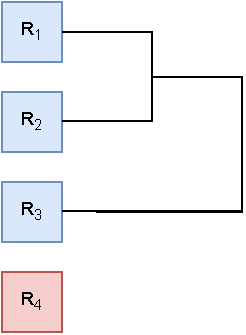
\includegraphics[width=0.25\textwidth]{dendrogram.pdf}
    \end{center}
    \caption{Graphische Veranschaulichung der gebildeten Cluster.}
    \label{fig:Dendrogram}
\end{figure}

\clearpage
\section{Related Work Analyse}
\label{3-RelatedWork}
\ac{DTW} kommt in vielen Arbeiten als Distanz-Metrik zum Einsatz.
Im Folgenden wird eine Auswahl dieser Veröffentlichungen und deren Einfluss auf diese Bachelorarbeit beschrieben.

\citet{wahyuni_motion_2021} entwickeln ein Erkennungssystem für Gesten.
Dabei wird eine Kinect-Kamera genutzt, um die Bewegungen aufzuzeichnen.
Es kommt eine Form des \ac{DTW}-Algorithmus zum Einsatz, um die Gesten zu erkennen.
Für den Vergleich von Bewegungsabläufen werden die x- und y-Koordinaten von sechs Körperpunkten genutzt.
Dabei liegen zu jeder bekannten Bewegung jeweils Referenzwerte für den Vergleich mit den aktuellen Werten vor.
Für die Entscheidung, ob eine betrachtete Bewegung zu einer Kategorie gehört oder nicht, sind die Kosten entscheidend.
Für das Ende des Clusterings wird ein Threshold definiert.
Liegt der berechnete Wert über diesem, wird die Bewegung verworfen.
Falls sie geringer sind, wird der Ablauf in die Kategorie einsortiert.
Die Definition von geeigneten Threshold-Werten für die Differenz zwischen Datenreihen
wird auch im späteren Verlauf dieser Arbeit relevant.
So kann entschieden werden, ob Cluster weiter zusammengeführt werden sollten oder nicht.
\citet{yu_dynamic_2019} nuzten \ac{DTW}, um physische Rehabilitationsübungen mithilfe eines Kinect-Sensors zu bewerten.
Dabei wird zunächst die Ähnlichkeit zwischen den Bewegungsabläufen des Nutzers und des Trainers berechnet.
Als Eingabeattribute werden hier acht sogenannte Knochenvektoren des menschlichen Skeletts und dessen Körperorientierung verwendet.
Ein Knochen, der zwischen zwei Gelenkpunkten liegt, wird als 3D-Vektor im Raum interpretiert.
Die Summe der Winkeldifferenzen zwischen allen korrespondierenden Knochenvektoren der beiden Bewegungsreihen dient
als Distanz-Metrik.
Die Ergebnisse zeigen, dass \ac{DTW} effektiv eingesetzt werden kann,
um automatisiert Bewegungsabläufe mit Vorlagen zu vergleichen und diese somit zu bewerten.
Im Kontext der Interaktion mit Wandbildschirmen können unterschiedliche Eingabewerte interessant sein.
In dieser Bachelorarbeit sollen die Attribute für den Vergleich, daher nicht bei der Implementierung festgelegt werden.
Stattdessen sollen sie frei konfigurierbar sein,
damit der Anwender das Clustering je nach Fragestellung mit verschiedenen Attributen durchführen kann.
Keines der in der Literatur gezeigten Systeme liefert eine derartige Funktionalität.
\citet{mohammadzade_dynamic_2021} nutzen \ac{TSD}-Informationen für eine Überwachung von alltäglichen menschlichen Aktivitäten.
Jede Aktion wird durch eine mehrdimensionale Time-Series repräsentiert,
wobei eine Dimension jeweils der Position eines Skelettpunkts im Verlauf der Zeit entspricht.
Im vorliegenden Ansatz wird jeder Bewegungsklasse genau eine Referenzbewegung zugeordnet.
Die Daten werden entsprechend mit diesen Referenzen verglichen.
Dadurch sind viel weniger Vergleiche nötig als bei anderen \ac{DTW}-Methoden,
wodurch die Rechenkomplexität abnimmt.
Allerdings sind dafür vordefinierte Klassen mit teils künstlich erzeugten Beispielbewegungen notwendig.
Wesentliches Ziel dieser Bachelorarbeit ist es allerdings dazu beizutragen, neue Informationen
über mögliche Interaktionsverhalten mit interaktiven Wandbildschirmen zu gewinnen.
Eine Definition im Voraus ist für dieses Szenario nicht zielführend.
Daher soll ein Clustering-Verfahren implementiert werden,
welches ohne vordefinierte Kategorien funktioniert.
\citet{hautamaki_time-series_2008} vergleichen experimentell einige \ac*{TSD} Clustering-Verfahren
mit \ac{DTW} als Distanzmetrik.
Unter anderem auch hierarchisches Clustering.
Hier werden zunächst alle Records als eigenes Cluster initialisiert.
Durch iterierte Anwendung von Merge-Operationen werden schrittweise zwei Cluster zusammengeführt,
die eine geringe Differenz aufweisen.
\citet{hautamaki_time-series_2008} prüfen die Zuverlässigkeit anhand mehrerer Experimente.
Unter anderem verwenden sie Sprachdaten, die ebenfalls zu den \ac{TSD} gehören.
Die Evaluation zeigt, dass hierarchisches Clustering in Kombination mit \ac{DTW} erfolgreich eingesetzt werden kann.
Ein Versuch im Kontext von Bewegungsdaten erfolgt in \citet{hautamaki_time-series_2008} allerdings nicht.

\section{Einsatz im Kontext von Kinect-Bewegungsdaten}
\label{3-Einsatz}
Wie bereits erwähnt handelt es sich bei den vorliegenden Kinect-Daten um \ac{TSD}.
\citet{warren_liao_clustering_2005} und \citet{aghabozorgi_time-series_2015} weisen darauf hin,
dass besonders die verwendete Distanzmetrik entscheidend ist,
um diesen Datentyp sinnvoll in Kategorien einteilen zu können.
Die vorgestellten Arbeiten in \autoref{3-RelatedWork} zeigen,
dass hierarchisches Clustering in Kombination mit \ac{DTW} ein vielversprechender Ansatz sein kann.
Da die Daten in Textdateien vorliegen, ist eine Komponente im System nötig,
die diese Informationen ausliest und in geeigneten Objekten der genutzten Programmiersprache abspeichert.
Von besonderer Bedeutung ist zudem die Wahl geeigneter Attribute.
Die Daten enthalten viele Werte, die mehr oder weniger interessant für die Kategorisierung sein können.
Welche Werte für eine Analyse relevant sind, muss im Einzelfall überprüft werden.
Die Wahl der genutzten Attribute muss also vom Nutzer definiert werden können.
So kann das Tool effektiv genutzt werden, um nach wiederkehrenden Abläufen in den Daten zu suchen.
Der zu definierende Threshold kann je nach Daten unterschiedlich ausfallen
und sollte daher ebenfalls von Nutzer konfiguriert werden können.
Abschließend ist die große Menge der Daten zu erwähnen.
\citet{aghabozorgi_time-series_2015} weisen darauf hin,
dass \ac{DTW} weniger performant ist als herkömmliche Metriken wie die euklidische Distanz.
Gegebenenfalls müssen die Daten vor der Nutzung geeignet gefiltert werden.
Diese Filterung ist allerdings nicht Bestandteil dieser Bachelorarbeit,
da sie deren Rahmen sprengen würde.
Für die Evaluation in \autoref{chapter6} wurden bereits gefilterte Daten bereitgestellt.